

\chapter{Förster Resonant Energy Transfer -- FRET}

\textit{spektral, fl. Lifetime, ensemble, JK dyade
}
\textit{Wie groß ist der Förster-Radius des Paares? Wie groß ist die Transfer-Effizient in dieser Dyade?
}


%\section{Experiment}



\section{6.1. Förster-Theorie  (FRET)\protect\footnote{Parson, Kap. 7.2, Simon Biberger}\hfill ***} 

\textit{Die Theorie von Förster beschreibt  den inkohärenten und
strahlungslosen Transfer  von Energie von einem Flurophor zu
einem eng benachbarten.}\\
Eine Möglichkeit, damit ein angeregtes Molekül in den Grundzustand gelangt, ist, indem diese Energie auf ein anderes Molekül übertragen wird. Dies wird Resonanz-Energie-Transfer genannt.
Zu Beginn sollen zwei benachbarte, aber nicht wechselwirkende Moleküle 1 und 2 betrachtet werden. Deren Hamilton-Operator lautet dann
\begin{equation*}
    H = H_1 + H_2
\end{equation*}
und die zugehörige Gesamt-Wellenfunktion für den Grundzustand ist das Produkt der beiden Einzel-Wellenfunktionen.
\begin{equation*}
    \Psi_{Ges} = \Phi_{1a} \chi_{1a}\cdot \Phi_{2a} \chi_{2a}
\end{equation*}
Ist nun eines der beiden Moleküle angeregt, wird die Gesamt-Wellenfunktion zu:
\begin{equation*}
    \Psi_{Ges} = C_1 \Phi_{1b} \chi_{1b}\cdot \Phi_{2a} \chi_{2a} + C_2 \Phi_{1a} \chi_{1a}\cdot \Phi_{2b} \chi_{2b}
\end{equation*}
Dabei stehen a und b jeweils für den Grund- bzw. angeregten Zustand und die Faktoren $C_1$ bzw. $C_2$ repräsentieren die Wahrscheinlichkeit, dass das Molekül angeregt ist. Dabei gilt $|C_1|^2 + |C_2|^2 = 1$.
Bei der Förster-Theorie wird nun eine Wechselwirkung zwischen den Molekülen zugelassen und der Hamilton-Operator lautet:
\begin{equation*}
    H_{Ges} = H_1 + H_2 + H_{21}
\end{equation*}
Startet man zur Zeit t\,=\,0 mit $C_1$\,=\,1 und $C_2$\,=\,0, lässt sich $C_2$ über zeitabhängige Störungstheorie bestimmen:
\begin{equation}
    C_2 = H_{21}\frac{1 - exp\left[\frac{i(E_2 - E_1)t}{\hbar}\right]}{E_2 - E_1}
    \label{c2}
\end{equation}
Aus Gleichung \ref{c2} kann sofort die Resonanz-Bedingung für den Energieunterschied zwischen Molekül 1 und 2 abgeleitet werden. $C_2$ hat nur einen signifikanten Betrag, wenn der Energieunterschied möglichst klein ist.
\begin{figure}
\label{Resonanz}
\center
    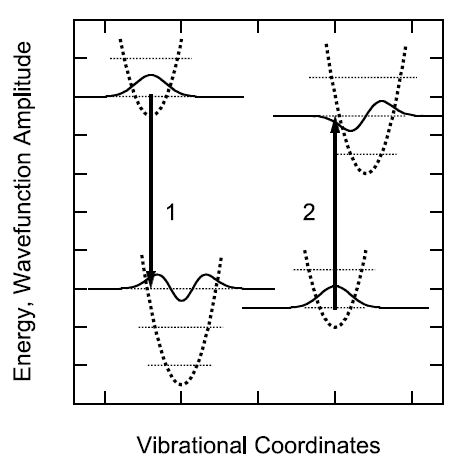
\includegraphics[width = 0.7 \textwidth]{\currfiledir/FRET.JPG}
    \caption{Der Resonanz-Energie-Transfer benötigt gekoppelte vibronische Übergänge nach oben und unten. Die Energie, die das Molekül 1 verliert, muss von Molekül 2 aufgenommen werden, sodass die Energie insgesamt erhalten bleibt. Außerdem müssen die zugehörigen Frank-Condon-Faktoren für die Übergänge ungleich null sein.}
\end{figure}

Die Gesamt-Rate für den Energie-Transfer kann mithilfe Fermis Goldener Regel bestimmt werden:
\begin{equation*}
    k_{rt} = \frac{2\pi}{\hbar} \cdot \int_{-\infty}^{+\infty} |H_{21}|^2 \rho_{s2}(E_1) \rho_{s1}(E_1) dE_1,
\end{equation*}
wobei mit $\rho_{si}$ die Zustandsdichten von Molekül 1 und 2 bezeichnet werden.

\section{6.2. FRET an einzelnen Molekülen zur Abstandsmessung\protect\footnote{Parson, Kap. 7.2 und 7.3}\hfill **} 

Die starke Abstandsabhängigkeit von FRET wird benutzt, um
die relative räumliche Lage von Marker-Fluorophoren
beispielsweise in Proteinen zu bestimmen.

Die Energieübertragung von einem angeregten Fluorophor auf ein anderes kann mit der Theorie des Förster-Resonanzenergietransfers beschrieben werden. Der Energieübertrag findet dabei strahlungslos über eine Dipol-Dipol-Wechselwirkung statt. Die Ratenkonstante $k_{rt}$ für diesen Übergang wird dabei wie folgt definiert:
\begin{equation}
    k_{rt}=\left( \frac{9000 ln(10)\kappa^2c^4\Phi}{128\pi^5n^4N_A\tau} \right) |R_{21}|^{-6}J ,
\end{equation}
wobei $\kappa$ der Orientierungsfaktor, $\Phi$ und $\tau$ die Quantenausbeute sowie Lebensdauer des Donors, $R_{21}$ der Abstand zwischen Donor und Akzeptor und J ein Überlappintegral zwischen dem Absorptions und Emissionsspektrum der beteiligten Fluorophore ist. Der Orientierungsfaktor $\kappa$ gibt die Ausrichtung der beiden als Dipole angenommen wechselwirkenden Partner an und kann Werte zwischen $-2$ und $2$ annehmen (s. Abb. \ref{KappaFaktor}). 
\begin{figure}
\label{KappaFaktor}
\center
    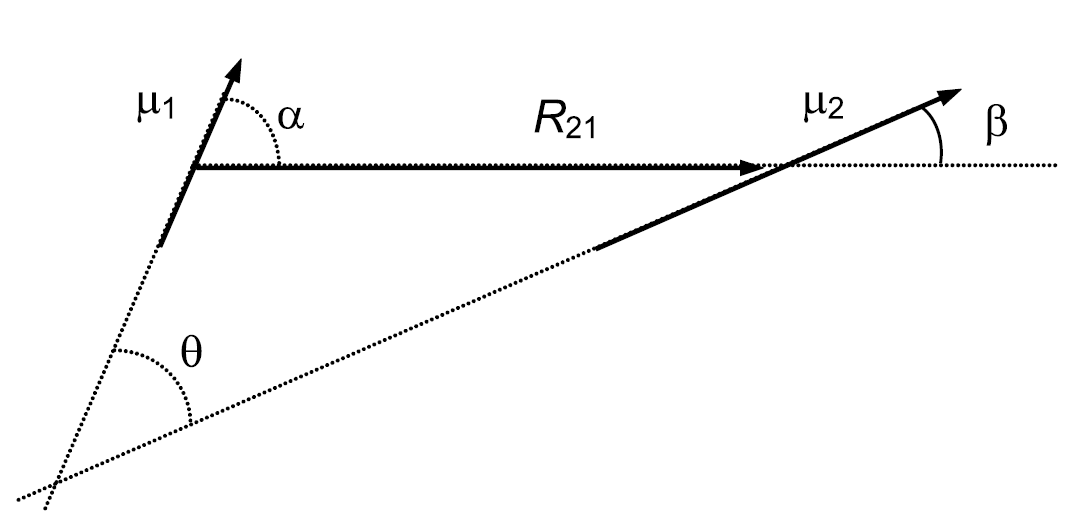
\includegraphics[width = 0.5 \textwidth]{\currfiledir/FretKappa.png}
    \caption{Skizze zur Lage der Winkel und des Abstandes der Dipole. Der Orientierungsfaktor $\kappa$ wird beschrieben durch: $\kappa=\cos(\theta)-3 \cos (\alpha)\cos (\beta)$}
\end{figure}
Die Gleichung für die Ratenkonstante wird auch oft in der verkürzten Form angegeben
\begin{equation}
\label{eq:fret}
    k_{rt}=\tau^{-1}(|R_{21}|/R_0)^{-6}
\end{equation}
mit dem Förster Radius $R_0$. Dieser gibt den Abstand an, bei welchem die Effizienz\footnote{Die Effizienz $E$ ist definiert als $E=\frac{1}{1+(r/R_0)^6}$ } des Energietransfer zu 50\% erfolgt.\par
Um mittels Fret den Abstand zwischen zwei Molekülen zu bestimmen, muss zunächst die Ratenkonstante $k_{rt}$ aus den Fluoreszenzausbeuten in Anwesenheit $\Phi$ und Abweseheit des Akzeptors $\Phi_q$ über folgende Formel berechnet werden 
\[ \frac{\Phi}{\Phi_q}=1+k_{rt}\tau .\]
Ist das Produkt aus $k_{rt}\tau$ und der Förster-Radius bekannt, kann der Abstand $|R_{21}|$ aus Gleichung \ref{eq:fret} errechnet werden.




\printbibliography[segment=\therefsegment,heading=subbibliography]
